
\section{Protocolo\label{subsec:Protocolo}}

Esta seção apresenta o protocolo do OpenDevice. As principais características
do protocolo é que ele foi projetado para ser um protocolo aberto,
leve, simples, de fácil implementação, legível para humanos e voltado
para dispositivos com restrições de memória e processamento, como
por exemplo, microcontroladores (AVR 8-bits, 2Kb de RAM).

O protocolo é baseado em ASCII (assim como o HTTP), orientado a mensagens/comandos
e assíncrono. Surgiu de algumas influências do protocolo MIDI (formato
usado para comunicação com instrumentos musicais) e do protocolo REST
na sua estrutura básica. 

O protocolo foi projetado para permitir a abstração, controle de dispositivos
(atuadores), realizar a leitura de sensores e ser de fácil extensão,
mas não limitado a isto. Ele pode ser utilizado em conjunto com outros
protocolos, como WebSocket e MQTT, e com outras tecnologias de comunicação,
como: USB, Bluetooth, Ethernet, Wi-Fi, etc. 


\subsection{Formato da Mensagem}

Os comandos do OpenDevice possuem um ``cabeçalho'' fixo, contento
o tipo do comando (\emph{CommandType}) e o ID do comando, em seguida,
o bloco \emph{``Command Extension}'', que varia de acordo com o
tipo de comando. 

\begin{figure}[H]
\begin{centering}
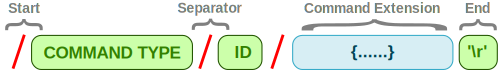
\includegraphics[width=0.8\linewidth]{Imagens/Cap_4/protocol_spec}
\par\end{centering}
\caption{Formato do protocolo OpenDevice \label{fig:protocol_spec}}
\end{figure}

\begin{itemize}
\item O \textbf{tipo do comando} define a estrutura do bloco ``\emph{Command
Extension}''. Os tipos suportados estão definidos na tabela \ref{tab:CommandType}. 
\item O \textbf{ID} do comando é numérico, sequencial e gerenciado pela
aplicação cliente. Ele serve para a aplicação identificar o retorno(resposta)
de algum comando enviado. Quando atinge seu valor máximo a contagem
reinicia.
\item Os blocos do comando são separados através do caractere ``/''.
\item O comando finaliza com o terminador ``\textbackslash{}r'' (Carriage
return).
\end{itemize}
\noun{Observação:} Na implementação atual do firmware, tanto o ``tipo
do comando'' quanto o ``id'', são armazenados em varáveis de 8bits
(uint8\_t / byte), limitando a valores na faixa de 0 a 255. Porém,
os mesmos são parametrizados podendo escolher outros tipos como: uint16\_t
ou uint32\_t.

\subsubsection{Convenções e pontos em aberto}

Algumas convenções foram adotadas para determinar observações, e destacar
pontos em aberto. Caso o texto apresente ``{[}{*}Numero{]}'', significa
que deve ser verificado as observações abaixo:
\begin{itemize}
\item Observação {[}{*}1{]}\noun{:} Na implementação atual do firmware,
o ``DeviceID'' é armazenado em uma variável de 8bits (byte), porém,
o tipo é parametrizável.
\item Observação {[}{*}2{]}\noun{: }Significa que o parâmetro ou tipo é
configurável. 
\item Observação {[}{*}3{]}\noun{:} Significa que a versão atual do firmware
não implementa o recurso.
\end{itemize}

\subsection{Tipos de Comandos}

A tabela \ref{tab:CommandType}, apresenta os tipos de comandos suportados.

\begin{table}[H]
\noindent\resizebox{\textwidth}{!}{
\begin{centering}
\begin{tabular}{|c|l|c|l|}
\hline 
Código & Tipo de Comando & Ref. & Formato\tabularnewline
\hline 
\hline 
1 & DIGITAL & \ref{subsec:DIGITAL} & {[}\#/\#{]}/\{DeviceID\}/\{value\}\tabularnewline
\hline 
2 & ANALOG & \ref{subsec:ANALOG} & {[}\#/\#{]}/\{DeviceID\}/\{value\}\tabularnewline
\hline 
3 & NUMERIC & \ref{subsec:NUMERIC} & {[}\#/\#{]}/\{DeviceID\}/\{value\}\tabularnewline
\hline 
4...9 & {[}Reservado{]} &  & –\tabularnewline
\hline 
10 & COMMAND\_RESPONSE & \ref{subsec:COMMAND_RESPONSE} & {[}\#/\#{]}/\{status\}/\{DeviceID?\}\tabularnewline
\hline 
11 & SET\_PROPERTY & \ref{subsec:SET_PROPERTY} & {[}\#/\#{]}/\{DeviceID\}/\{property\}/\{value\}\tabularnewline
\hline 
12 & GET\_PROPERTIES & \ref{subsec:GET_PROPERTIES} & {[}\#/\#{]}/\{DeviceID\}\tabularnewline
\hline 
13 & GET\_PROPERTIES\_RESPONSE & \ref{subsec:GET_PROPERTIES_RESPONSE} & {[}\#/\#{]}/\{DeviceID\}/{[}\{property1:value\},...,N{]}\tabularnewline
\hline 
14 & ACTION & \ref{subsec:ACTION} & {[}\#/\#{]}/\{DeviceID\}/\{action\}/{[}\{value1?\},...,\{valueN\}{]}\tabularnewline
\hline 
15 & GET\_ACTIONS & \ref{subsec:GET_ACTIONS} & {[}\#/\#{]}/\{DeviceID\}\tabularnewline
\hline 
16 & GET\_ACTIONS\_RESPONSE & \ref{subsec:GET_ACTIONS_RESPONSE} & {[}\#/\#{]}/\{DeviceID\}/{[}\{action1\},\{actionN\}{]}\tabularnewline
\hline 
16...19 & {[}Reservado{]} &  & –\tabularnewline
\hline 
20 & PING\_REQUEST & \ref{subsec:PING_REQUEST} & {[}\#/\#{]}{[}somente cabeçalho{]}\tabularnewline
\hline 
21 & PING\_RESPONSE & \ref{subsec:PING_RESPONSE} & {[}\#/\#{]}{[}somente cabeçalho{]}\tabularnewline
\hline 
22 & DISCOVERY\_REQUEST & \ref{subsec:DISCOVERY_REQUEST} & {[}\#/\#{]}{[}somente cabeçalho{]}\tabularnewline
\hline 
23 & DISCOVERY\_RESPONSE & \ref{subsec:DISCOVERY_RESPONSE} & {[}\#/\#{]}/\{name\}/\{port\}/\{deviceLength\}\tabularnewline
\hline 
24...29 & {[}Reservado{]} &  & –\tabularnewline
\hline 
30 & GET\_DEVICES & \ref{subsec:GET_DEVICES} & {[}\#/\#{]}/\{DeviceID?\}/\{value?\}\tabularnewline
\hline 
31 & GET\_DEVICES\_RESPONSE & \ref{subsec:GET_DEVICES_RESPONSE} & {[}\#/\#{]}/{[}\{DeviceInfo1\},\{DeviceInfoN?{]}\tabularnewline
\hline 
32 & DEVICE\_ADD & \ref{subsec:DEVICE_ADD} & {[}\#/\#{]}/\{DeviceInfo\}\tabularnewline
\hline 
33 & DEVICE\_DEL & \ref{subsec:DEVICE_DEL} & {[}\#/\#{]}/\{DeviceID?\}\tabularnewline
\hline 
41..100 & {[}Reservado{]} &  & \tabularnewline
\hline 
\end{tabular}
\par\end{centering}
}

\caption{Tipos de comandos do protocolo\label{tab:CommandType}}
\end{table}


\subsection{Comando: DIGITAL\label{subsec:DIGITAL}}

Este comando permite controlar os dispositivos digitais (atuadores)
ou notificar alguma mudança no estado/valor de um sensor. O comando
adiciona dois blocos adicionais: DeviceID e Value (Figura \ref{fig:protocol_cmd}). 

Ao enviar um comando para um dispositivo, por exemplo, ligar lâmpada,
o dispositivo deve retornar uma resposta (geralmente assíncrona),
com o status do comando. 

O formato da resposta é definida em \emph{``}\nameref{subsec:COMMAND_RESPONSE}'',
onde o ID da resposta será o mesmo ID do comando enviado.

\begin{figure}[H]
\begin{centering}
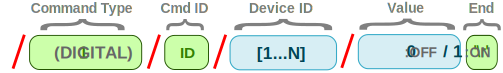
\includegraphics[width=0.8\linewidth]{Imagens/Cap_4/protocol_cmd_digital}
\par\end{centering}
\caption{Comando: DIGITAL\label{fig:protocol_cmd}}
\end{figure}

\begin{table}[H]
\begin{centering}
\begin{tabular}{|c|c|l|}
\hline 
Parâmetro & Tipo & Descrição\tabularnewline
\hline 
\hline 
DeviceID & byte {[}{*}1{]} & Identificador único que representa o dispositivo\tabularnewline
\hline 
Value & bool & 0 (Desligar / Desligado) ou 1 (Ligar / Ligado)\tabularnewline
\hline 
\end{tabular}
\par\end{centering}
\caption{Parâmetros - Comando: DIGITAL}
\end{table}


\subsection{Comando: ANALOG\label{subsec:ANALOG}}

Obedece o formado do ``\nameref{subsec:DIGITAL}'', mudando apenas
o tipo do comando, no caso 2, e o tipo de dado do bloco ``\emph{Value}'',
que pode aceitar valores do tipo \emph{``unsigned long}'', com tamanho
de 32 bits (4 bytes). 

Este comando pode ser utilizado tanto para sensores como para atuadores,
no caso de sensores, ele é utilizado para notificar um mudança de
estado (já que sensores são apenas para ``leitura'').

O formato da resposta é definida em \emph{``}\nameref{subsec:COMMAND_RESPONSE}'',
onde o ID da resposta será o mesmo ID do comando enviado.

\subsection{Comando: NUMERIC\label{subsec:NUMERIC}}

Obedece o formado do ``\nameref{subsec:ANALOG}''. Este comando
é utilizado em conjunto com os dispositivos (principalmente sensores)
do tipo \emph{NUMERIC}, que permitem o envio de informações repetidas.
Um exemplo, o sensor RFID, que gera um evento toda vez que uma etiqueta
é lida, mesmo sendo a mesma etiqueta.

\subsection{Reposta: COMMAND\_RESPONSE\label{subsec:COMMAND_RESPONSE}}

Representa a resposta de um determinado comando. As respostas são
associadas ao comando que a originou (requisição), através do atributo
``ID'' do cabeçalho fixo. Adicionalmente os comandos que referenciam
um dispositivo, na resposta, será incluído o mesmo ``DeviceID''
do comando da ``requisição''.

\begin{table}[H]
\begin{centering}
\begin{tabular}{|c|c|c|}
\hline 
\prth HEADER & \prtv Status & \prtv DeviceID\tabularnewline
\hline 
\end{tabular}
\par\end{centering}
\caption{Reposta: COMMAND\_RESPONSE}
\end{table}

\begin{table}[H]
\begin{centering}
\begin{tabular}{|c|c|l|}
\hline 
Parâmetro & Tipo & Descrição\tabularnewline
\hline 
\hline 
ID & byte {[}{*}2{]} & Mesmo ID enviado na requisição\tabularnewline
\hline 
Status & byte & Obedece aos valores da tabela: \ref{tab:CommandStatusResp}\tabularnewline
\hline 
DeviceID & byte {[}{*}1{]} (Opcional) & Mesmo ID enviado na requisição\tabularnewline
\hline 
\end{tabular}
\par\end{centering}
\caption{Parâmetros - Comando: COMMAND\_RESPONSE\label{tab:CommandStatusResp-1-1}}
\end{table}

\begin{table}[H]
\begin{centering}
\begin{tabular}{|c|c|}
\hline 
Status & Código\tabularnewline
\hline 
\hline 
SUCCESS & 200\tabularnewline
\hline 
NOT\_FOUND & 404\tabularnewline
\hline 
BAD\_REQUEST & 400\tabularnewline
\hline 
\textcolor{red}{UNAUTHORIZED {[}{*}3{]}} & 401\tabularnewline
\hline 
\textcolor{red}{FORBIDDEN {[}{*}3{]}} & 403\tabularnewline
\hline 
\textcolor{red}{PERMISSION\_DENIED {[}{*}3{]}} & 550\tabularnewline
\hline 
INTERNAL\_ERROR & 500\tabularnewline
\hline 
NOT\_IMPLEMENTED & 501\tabularnewline
\hline 
\end{tabular}
\par\end{centering}
\caption{Status da resposta do comando\label{tab:CommandStatusResp}}
\end{table}


\subsection{Comando: SET\_PROPERTY\label{subsec:SET_PROPERTY}}

Comando utilizado para atualizar alguma propriedade do dispositivo.
O formato da resposta é definido em \emph{``}\nameref{subsec:COMMAND_RESPONSE}''.

\begin{table}[H]
\begin{centering}
\begin{tabular}{|c|c|c|c|}
\hline 
\prth HEADER & \prtv DeviceID & \prtv property & \prtv value\tabularnewline
\hline 
\end{tabular}
\par\end{centering}
\caption{Comando: SET\_PROPERTY}
\end{table}

\begin{table}[H]
\begin{centering}
\begin{tabular}{|c|c|l|}
\hline 
Parâmetro & Tipo & Descrição\tabularnewline
\hline 
\hline 
DeviceID & byte {[}{*}1{]} & Identificador único que representa o dispositivo\tabularnewline
\hline 
property & String & Propriedade a ser alterada\tabularnewline
\hline 
value & String & Valor da propriedade\tabularnewline
\hline 
\end{tabular}
\par\end{centering}
\caption{Parâmetros: SET\_PROPERTY}
\end{table}


\subsection{Comando: GET\_PROPERTIES\label{subsec:GET_PROPERTIES}}

Comando utilizado para recuperar a lista de propriedades do dispositivo
e seus respectivos valores. O formato da resposta é definido em \emph{``}\nameref{subsec:GET_PROPERTIES_RESPONSE}''

\begin{table}[H]
\begin{centering}
\begin{tabular}{|c|c|}
\hline 
\prth HEADER & \prtv DeviceID\tabularnewline
\hline 
\end{tabular}
\par\end{centering}
\caption{Comando: GET\_PROPERTIES}
\end{table}

\begin{table}[H]
\begin{centering}
\begin{tabular}{|c|c|l|}
\hline 
Parâmetro & Tipo & Descrição\tabularnewline
\hline 
\hline 
DeviceID & byte {[}{*}1{]} & Identificador único que representa o dispositivo\tabularnewline
\hline 
\end{tabular}
\par\end{centering}
\caption{Parâmetros: GET\_PROPERTIES}
\end{table}


\subsection{Comando: GET\_PROPERTIES\_RESPONSE\label{subsec:GET_PROPERTIES_RESPONSE}}

Resposta do comando ``\emph{GET\_PROPERTIES}'', com a lista de propriedades
do dispositivo. A lista é retornada no formato de um Array, e os elementos
no formato: ``Propriedade:Valor''.

\begin{table}[H]
\begin{centering}
\begin{tabular}{|c|c|c|}
\hline 
\prth HEADER & \prtv DeviceID & \prtv{[}property:value,...,propertyN:value{]}\tabularnewline
\hline 
\end{tabular}
\par\end{centering}
\caption{Comando: GET\_PROPERTIES\_RESPONSE}
\end{table}

\begin{table}[H]
\begin{centering}
\begin{tabular}{|c|c|l|}
\hline 
Parâmetro & Tipo & Descrição\tabularnewline
\hline 
\hline 
DeviceID & byte {[}{*}1{]} & Identificador único que representa o dispositivo\tabularnewline
\hline 
property & String & Propriedade\tabularnewline
\hline 
value & String & Valor da propriedade\tabularnewline
\hline 
\end{tabular}
\par\end{centering}
\caption{Parâmetros: GET\_PROPERTIES\_RESPONSE}
\end{table}


\subsection{Comando: ACTION\label{subsec:ACTION}}

Comando usado para executar as ações definidas pelos dispositivos.
As ações podem receber uma lista de valores, que são especificados
em formato de Array. O formato da resposta é definido em \emph{``}\nameref{subsec:COMMAND_RESPONSE}''.

\begin{table}[H]
\begin{centering}
\begin{tabular}{|c|c|c|c|}
\hline 
\prth HEADER & \prtv DeviceID & \prtv action & \prtv{[}\{value1\},...,\{valueN\}{]}\tabularnewline
\hline 
\end{tabular}
\par\end{centering}
\caption{Comando: ACTION}
\end{table}

\begin{table}[H]
\begin{centering}
\begin{tabular}{|c|c|l|}
\hline 
Parâmetro & Tipo & Descrição\tabularnewline
\hline 
\hline 
DeviceID & byte {[}{*}1{]} & Identificador único que representa o dispositivo\tabularnewline
\hline 
action & String & Ação que deve ser executada\tabularnewline
\hline 
value & Array{[}String{]} (Opcional) & A lista de valores que a ação recebe\tabularnewline
\hline 
\end{tabular}
\par\end{centering}
\caption{Parâmetros: ACTION}
\end{table}


\subsection{Comando: GET\_ACTIONS\label{subsec:GET_ACTIONS}}

Comando utilizado para recuperar a lista de ações definidas para o
dispositivo. O formato da resposta é definido em \emph{``}\nameref{subsec:GET_ACTIONS_RESPONSE}''

\begin{table}[H]
\begin{centering}
\begin{tabular}{|c|c|}
\hline 
\prth HEADER & \prtv DeviceID\tabularnewline
\hline 
\end{tabular}
\par\end{centering}
\caption{Comando: GET\_ACTIONS}
\end{table}

\begin{table}[H]
\begin{centering}
\begin{tabular}{|c|c|l|}
\hline 
Parâmetro & Tipo & Descrição\tabularnewline
\hline 
\hline 
DeviceID & byte {[}{*}1{]} & Identificador único que representa o dispositivo\tabularnewline
\hline 
\end{tabular}
\par\end{centering}
\caption{Parâmetros: GET\_ACTIONS}
\end{table}


\subsection{Comando: GET\_ACTIONS\_RESPONSE\label{subsec:GET_ACTIONS_RESPONSE}}

Resposta do comando ``\emph{GET\_ACTIONS}'', com a lista de ações
do dispositivo. A lista é retornada no formato de um Array.

\begin{table}[H]
\begin{centering}
\begin{tabular}{|c|c|c|}
\hline 
\prth HEADER & \prtv DeviceID & \prtv {[}\{action1\},..,\{actionN\}{]}\tabularnewline
\hline 
\end{tabular}
\par\end{centering}
\caption{Comando: GET\_ACTIONS\_RESPONSE}
\end{table}

\begin{table}[H]
\begin{centering}
\begin{tabular}{|c|c|l|}
\hline 
Parâmetro & Tipo & Descrição\tabularnewline
\hline 
\hline 
DeviceID & byte {[}{*}1{]} & Identificador único que representa o dispositivo\tabularnewline
\hline 
action & Array{[}String{]} & Lista de ações do dispositivo\tabularnewline
\hline 
\end{tabular}
\par\end{centering}
\caption{Parâmetros: GET\_ACTIONS\_RESPONSE}
\end{table}


\subsection{Comando: PING\_REQUEST\label{subsec:PING_REQUEST}}

Comando enviado pelo firmware para notificar que está em funcionamento
e ao mesmo tempo monitora o status do middleware/aplicação. 

Este comando não possui parâmetros adicionais, apenas cabeçalho. O
formato da resposta é definido em \emph{``}\nameref{subsec:PING_RESPONSE}''

\subsection{Resposta: PING\_RESPONSE\label{subsec:PING_RESPONSE}}

Resposta para o comando ``PING\_REQUEST''. Este comando não possui
parâmetros adicionais, apenas cabeçalho.

\subsection{Comando: DISCOVERY\_REQUEST\label{subsec:DISCOVERY_REQUEST}}

Comando utilizado para realizar a descoberta de dispositivos (módulos)
em uma rede. Geralmente é enviado via \emph{broadcast}. Este comando
não possui parâmetros adicionais, apenas cabeçalho.

\subsection{Resposta: DISCOVERY\_RESPONSE\label{subsec:DISCOVERY_RESPONSE}}

Resposta com as informações de descoberta dos dispositivos (módulos)
. 

\begin{table}[H]
\begin{centering}
\begin{tabular}{|c|c|c|c|c|}
\hline 
\prth HEADER & \prtv name & \prtv type & \prtv deviceLength & \prtv port\tabularnewline
\hline 
\end{tabular}
\par\end{centering}
\caption{Comando: GET\_ACTIONS\_RESPONSE}
\end{table}

\begin{table}[H]
\begin{centering}
\begin{tabular}{|c|c|l|}
\hline 
Parâmetro & Tipo & Descrição\tabularnewline
\hline 
\hline 
name & String & Nome do dispositivo (módulo)\tabularnewline
\hline 
type & int & Identifica o tipo de dispositivo (NODE/MANAGER)\tabularnewline
\hline 
deviceLength & int & Quantidades de dispositivos que o módulo possui\tabularnewline
\hline 
port & int (Opcional) & Porta de conexão (apenas para TCP/WIFI)\tabularnewline
\hline 
\end{tabular}
\par\end{centering}
\caption{Parâmetros: DISCOVERY\_RESPONSE}
\end{table}


\subsection{Comando: GET\_DEVICES\label{subsec:GET_DEVICES}}

Comando usado para obter informações de um ou mais dispositivos. Os
campos 'DeviceID' e 'Valor' são opcionais e podem ser usados como
filtro para o comando. 

\begin{table}[H]
\begin{centering}
\begin{tabular}{|c|c|c|}
\hline 
\prth HEADER & \prtv DeviceID & \prtv Value\tabularnewline
\hline 
\end{tabular}
\par\end{centering}
\caption{Comando: GET\_DEVICES}
\end{table}

\begin{table}[H]
\begin{centering}
\begin{tabular}{|c|c|l|}
\hline 
Parâmetro & Tipo & Descrição\tabularnewline
\hline 
\hline 
DeviceID (Opcional) & byte {[}{*}1{]} & Informar o ID do dispositivo ou 0 para todos\tabularnewline
\hline 
Value (Opcional) & \emph{unsigned long} & Permite filtrar por valor ou 0 para todos\tabularnewline
\hline 
\end{tabular}
\par\end{centering}
\caption{Parâmetros: GET\_DEVICES}
\end{table}


\subsection{Resposta: GET\_DEVICES\_RESPONSE\label{subsec:GET_DEVICES_RESPONSE}}

Resposta do comando ``GET\_DEVICES'', com a lista de dispositivos
cadastrados. O bloco ``\emph{Command Extension}'', consiste em um
Array de objetos do ``\nameref{subsec:Objeto_DeviceInfo}'', separados
por ``,''. A quantidade de dispositivos deve ser inferida automaticamente.

\begin{table}[H]
\begin{centering}
\begin{tabular}{|c|c|}
\hline 
\prth HEADER & \prtv {[}DeviceInfo,...,DeviceInfoN{]}\tabularnewline
\hline 
\end{tabular}
\par\end{centering}
\caption{Resposta: GET\_DEVICES\_RESPONSE}
\end{table}

\begin{table}[H]
\begin{centering}
\begin{tabular}{|c|c|c|}
\hline 
Parâmetro & Tipo & Descrição\tabularnewline
\hline 
\hline 
ID & byte {[}{*}2{]} & Mesmo ID enviado da requisição\tabularnewline
\hline 
DeviceInfo & Array{[}DeviceInfo{]} & Lista dos atributos do \nameref{subsec:Objeto_DeviceInfo}\tabularnewline
\hline 
\end{tabular}
\par\end{centering}
\caption{Parâmetros - Resposta: GET\_DEVICES\_RESPONSE}
\end{table}


\subsection{Comando: DEVICE\_ADD\label{subsec:DEVICE_ADD}}

Comando utilizado para configurar dinâmicamente os dispositivos de
um módulo. O formato da resposta é definido em \emph{``}\nameref{subsec:COMMAND_RESPONSE}''.

\begin{table}[H]
\begin{centering}
\begin{tabular}{|c|c|}
\hline 
\prth HEADER & \prtv DeviceInfo\tabularnewline
\hline 
\end{tabular}
\par\end{centering}
\caption{Comando: DEVICE\_ADD}
\end{table}

\begin{table}[H]
\begin{centering}
\begin{tabular}{|c|c|l|}
\hline 
Parâmetro & Tipo & Descrição\tabularnewline
\hline 
\hline 
DeviceInfo & DeviceInfo & Lista dos atributos do \nameref{subsec:Objeto_DeviceInfo}\tabularnewline
\hline 
\end{tabular}
\par\end{centering}
\caption{Parâmetros: DEVICE\_ADD}
\end{table}


\subsection{Comando: DEVICE\_DEL\label{subsec:DEVICE_DEL}}

Comando utilizado deletar o(s) dispositiv(o) de um módulo. O formato
da resposta é definido em \emph{``}\nameref{subsec:GET_ACTIONS_RESPONSE}''

\begin{table}[H]
\begin{centering}
\begin{tabular}{|c|c|}
\hline 
\prth HEADER & \prtv DeviceID\tabularnewline
\hline 
\end{tabular}
\par\end{centering}
\caption{Comando: DEVICE\_DEL}
\end{table}

\begin{table}[H]
\begin{centering}
\begin{tabular}{|c|c|l|}
\hline 
Parâmetro & Tipo & Descrição\tabularnewline
\hline 
\hline 
DeviceID & byte {[}{*}1{]} (Opcioanl) & Informar o ID do dispositivo ou 0 para todos\tabularnewline
\hline 
\end{tabular}
\par\end{centering}
\caption{Parâmetros: DEVICE\_DEL}
\end{table}


\subsection{Tipo: DeviceInfo\label{subsec:Objeto_DeviceInfo}}

Representa as informações e um dispositivo. É representado como um
Array no seguinte formato: \inputencoding{latin9}\lstinline![ID, PIN, VALUE, TARGET, SENSOR, TYPE]!\inputencoding{utf8}.

\begin{table}[H]
\begin{centering}
\begin{tabular}{|c|c|l|}
\hline 
Atributo & Tipo & Descrição\tabularnewline
\hline 
\hline 
ID & byte {[}{*}2{]} & ID do dispositivo \tabularnewline
\hline 
PIN & byte & Pino que o dispositivo está vinculado\tabularnewline
\hline 
VALUE & unsigned long & Valor atual do dispositivo\tabularnewline
\hline 
TARGET & byte & Quando for sensor, representa outro dispositivo (Opcional)\tabularnewline
\hline 
SENSOR & bool & 0 para atuador, 1 para sensor\tabularnewline
\hline 
TYPE & byte & Tipo de dispositivo (Tabela \ref{tab:TipoDispositivo})\tabularnewline
\hline 
\end{tabular}
\par\end{centering}
\caption{Objeto: DeviceInfo}
\end{table}

\begin{table}[H]
\begin{centering}
\begin{tabular}{|c|c|}
\hline 
Código & Tipo\tabularnewline
\hline 
\hline 
1 & DIGITAL\tabularnewline
\hline 
2 & ANALOG\tabularnewline
\hline 
3 & NUMERIC\tabularnewline
\hline 
\end{tabular}
\par\end{centering}
\caption{Tipos de Dispositivos\label{tab:TipoDispositivo}}
\end{table}

